
\lecture{Confidence Intervals}{confidence-interval}
\section{Confidence Intervals}

\title{The Confidence Interval}
\subtitle{Introducing the Idea}

%\author{Kelly Black}
%\institute{Clarkson University}
\date{23 February 2015}

\begin{frame}
  \titlepage
\end{frame}

\begin{frame}
  \frametitle{Outline}
  \tableofcontents[hideothersubsections,sectionstyle=show/hide]
\end{frame}


\subsection{Clicker Quiz}

\iftoggle{clicker}{%
  \begin{frame}
    \frametitle{Clicker Quiz}

    You sample a random variable which has a mean of 2.1 and a
    standard deviation of 4.5. You take 30 samples, and the sample
    mean is 3.5. What is the value of the $z$-statistic? (The
    $z$-statistic is the value of $z^*$ associated with this sample
    mean.)

    \vfill

    \begin{tabular}{l@{\hspace{3em}}l@{\hspace{3em}}l@{\hspace{3em}}l}
      A: 0.31  & B: 0.78  & C: 1.70
    \end{tabular}

    \vfill
    \vfill
    \vfill

  \end{frame}
}

\subsection{The Confidence Interval}


\begin{frame}
  \frametitle{Problem!}

  We have a random variable, $X$. We want to know what its mean,
  $\mu$, or its standard deviation, $\sigma$, is. How do we figure
  this out?

  \vfill

  \only<2->
  {
    \begin{block}{Example}
      We run a capitol investment firm. Someone says that they need
      \$250,000 to start a restaurant. It this a reasonable amount?
    \end{block}
  }

  \vfill

\end{frame}


\begin{frame}{The Big Question}

  How do we estimate the mean of a random variable?
  
\end{frame}


\begin{frame}{Example}
  
  We call up ten random restaurant owners and ask them for the amount
  they needed to get started. We get the following amounts:
  \begin{tabular}{lllll}
    \$250,397 & \$241,621 & \$238,706 & \$249,276 & \$248,577 \\
    \$260,748 & \$268,647 & \$269,197 & \$232,603 & \$221,389
  \end{tabular}

  We then calculate a \textcolor{red}{\textit{sample mean}},
  \begin{eqnarray*}
    \bar{x} & = &
    \frac{250397+241621+238706+\cdots+232603+221389}{10}, \\
    & = & \$248,116.10\\
  \end{eqnarray*}
  This is our \textcolor{blue}{\textbf{estimate}} for the mean.
  
\end{frame}


\iftoggle{clicker}{%
  \begin{frame}
    \frametitle{Clicker Quiz}

    We call up ten random restaurant owners and ask them for the
    amount they needed to get started. We get the following amounts:
    \begin{tabular}{lllll}
    \$250,397 & \$241,621 & \$238,706 & \$249,276 & \$248,577 \\
    \$260,748 & \$268,647 & \$269,197 & \$232,603 & \$221,389
    \end{tabular}

    We then calculate a \textit{sample mean},
    \begin{eqnarray*}
      \bar{x} & = &
      \frac{250397+241621+238706+\cdots+232603+221389}{10}, \\
      & = & \$248,116.10\\
    \end{eqnarray*}

    Is this estimate close to the true mean?

    \vfill

    \begin{tabular}{l@{\hspace{3em}}l@{\hspace{3em}}l@{\hspace{3em}}l}
      A: Yes  & B: No  & C: Maybe??
    \end{tabular}

    \vfill
    \vfill
    \vfill

  \end{frame}
}

\begin{frame}{Stupid Coworker}
  
  One of your coworkers tries to suck up to the boss and also calls
  ten random restaurant owners and ask them for the amount they needed
  to get started. He got the following amounts:
  \begin{tabular}{lllll}
    \$237,031 & \$275,563 & \$255,643 & \$264,230 & \$251,355 \\
    \$257,822 & \$252,246 & \$252,851 & \$260,110 & \$247,164
  \end{tabular}

  The resulting \textit{sample mean} is
  \begin{eqnarray*}
    \bar{x} & = &
    \frac{237031+275563+255643+\cdots+260110+247164}{10}, \\
    & = & \$255,401.50\\
  \end{eqnarray*}

  \only<2->{\color{red}Which one of you is right?}
  
\end{frame}


\begin{frame}{Estimators}

  The only thing that we have is $\bar{x}$ and $s$. The problem is
  that these things are random variables.

  $\bar{x}$ is an \textcolor{red}{estimate} for the mean, $\mu$.

  $s$ is an \textcolor{red}{estimate} for the standard deviation, $\sigma$.

  \begin{definition}{Bias}
    \begin{itemize}
    \item If our estimator for a parameter is {\color{red}expected} to be less that
      the true value it has a \textit{\color{blue}negative bias.}
    \item If our estimator for a parameter is {\color{red}expected} to be more that
      the true value it has a \textit{\color{blue} positive bias.}
    \item If the {\color{red}expectation} of our estimator for a parameter is the
      same as the true value then it is \textit{\color{blue} unbiased.}
    \end{itemize}
  \end{definition}
  
  \vfill

\end{frame}

\begin{frame}{Estimator Of The Mean}

  \begin{definition}[Estimator of the mean]
    The sample mean is an estimator of the mean,
  \begin{eqnarray*}
    \bar{x} & = & \frac{x_1 + x_2 + x_3 + \cdots + x_{n}}{n}.
  \end{eqnarray*}    
  \end{definition}
  
  \vfill
  \vfill
  \vfill

\end{frame}


\begin{frame}{The Sample Mean}

\only<1>{\centerline{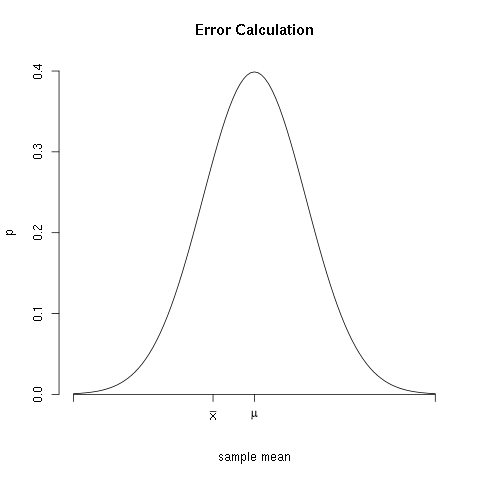
\includegraphics[width=6cm]{img/approximateMeanBlank}}}
\only<2>{\centerline{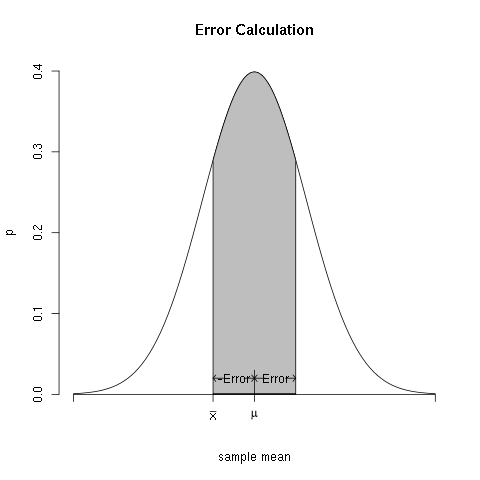
\includegraphics[width=6cm]{img/approximateMean}}}

Question: How close is $\bar{x}$ to $\mu$? 

Problem: We do not know what $\mu$ is!
  
\end{frame}


\begin{frame}{Confidence Interval}

  There is a probability of $1-\alpha$ that $\bar{x}$ is within the
  error of the true mean.

  \begin{columns}
    \column{.4\textwidth}

    \centerline{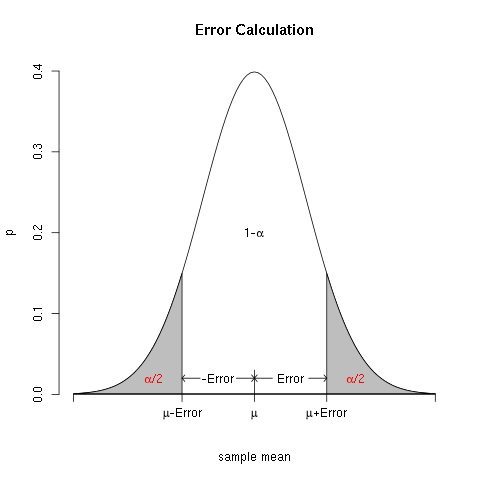
\includegraphics[width=4cm]{img/confidenceInterval}}

    \column{.6\textwidth}

    In practice we usually want one of the following things:
    \begin{itemize}
    \item Determine the value of the error for a given value of $\alpha$.
    \item Determine number of samples (N).
    \item Determine the probability that we are outside of the error bounds.
    \end{itemize}

  \end{columns}
  
\end{frame}


\begin{frame}{Confidence Interval}

  \begin{columns}
    \column{.4\textwidth}
    \centerline{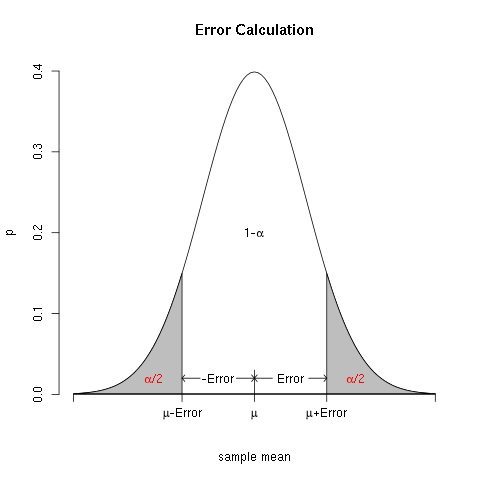
\includegraphics[width=4cm]{img/confidenceInterval}}

    \column{.6\textwidth}
    The key relationship:
    \begin{eqnarray*}
      p\lp \mu-\mathrm{error} \leq \bar{x} \leq \mu + \mathrm{error}\rp
      & = & 1-\alpha
    \end{eqnarray*}
    or
    \begin{eqnarray*}
      p\lp \bar{x} \leq \mu-\mathrm{error} \rp & = & \frac{\alpha}{2},
    \end{eqnarray*}
    and
    \begin{eqnarray*}
      z^* & = & \frac{-\mathrm{error}}{\sigma/n}.
    \end{eqnarray*}

    $z^*$ is the \textcolor{red}{critical $z$-statistic}.

  \end{columns}

\end{frame}



\iftoggle{clicker}{%
  \begin{frame}
    \frametitle{Clicker Quiz}


    \centerline{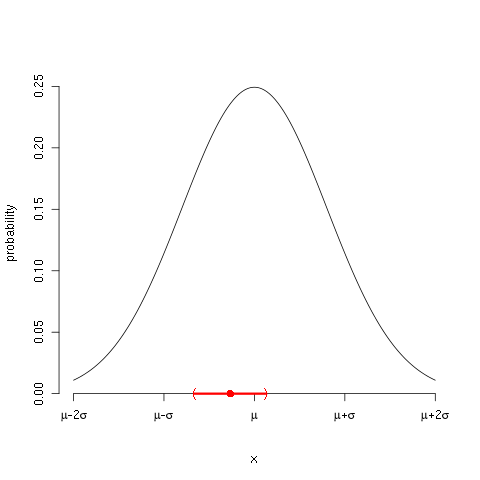
\includegraphics[width=6cm]{img/week8DistConfInterval}}
    If the value of $\alpha$ is increased does the length of the
    ``error'' increase or decrease?  \vfill

    \begin{tabular}{l@{\hspace{3em}}l@{\hspace{3em}}l@{\hspace{3em}}l}
      A: Increase  & B: Decrease
    \end{tabular}

    \vfill
    \vfill
    \vfill

  \end{frame}
}



\begin{frame}
  \frametitle{Estimator for the mean}


  \only<1>{\centerline{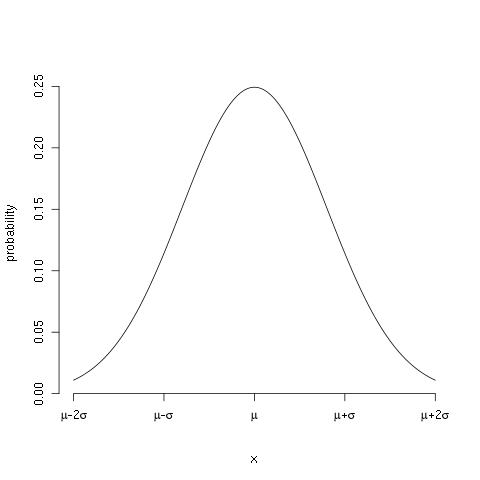
\includegraphics[width=6cm]{img/week8Dist}}}
  \only<2>{\centerline{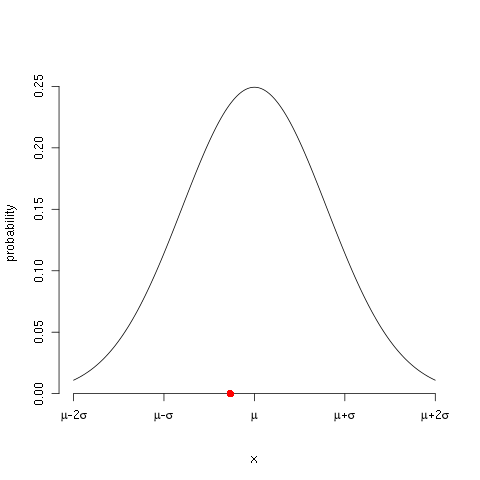
\includegraphics[width=6cm]{img/week8DistSample}}}
  \only<3>{%
    \centerline{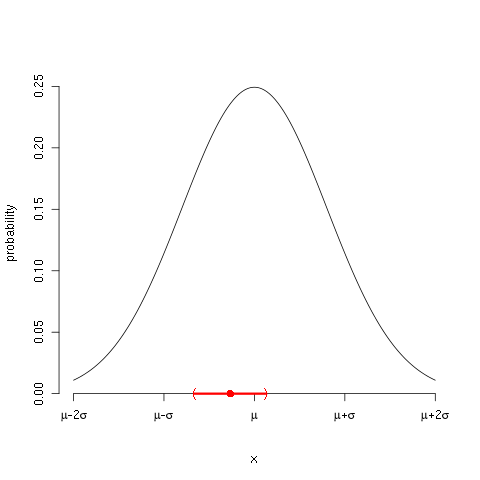
\includegraphics[width=6cm]{img/week8DistConfInterval}}

    We want to determine the probability that
    \begin{eqnarray*}
      \bar{x}-\mathrm{error} \leq \mu \leq \bar{x}+\mathrm{error}.
    \end{eqnarray*}

  }

\end{frame}

\begin{frame}{Confidence Interval}

  \begin{columns}
    \column{.3\textwidth}

    \centerline{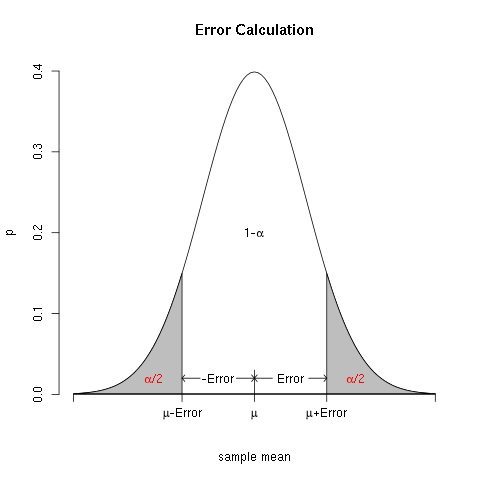
\includegraphics[width=4cm]{img/confidenceInterval}}

    \column{.7\textwidth}

    We usually want one of the following things:
    \begin{itemize}
    \item Given $N$ and $\alpha$ calculate the error.
    \item Given $N$ and the error calculate $\alpha$.
    \item Given $\alpha$ and the error calculate $N$.
    \end{itemize}

  \end{columns}
  
\end{frame}


\begin{frame}{The Relationship Between $N$, error, and $\alpha$}

  \only<1-2>%
  {
    We want to determine the probability that
    \begin{eqnarray*}
      \bar{x}-\mathrm{error} \leq \mu \leq \bar{x}+\mathrm{error}.
    \end{eqnarray*}
    but we can work with the relationship
    \begin{eqnarray*}
      p\lp \mu-\mathrm{error} \leq \bar{x} \leq \mu + \mathrm{error}\rp
      & = & 1-\alpha      
    \end{eqnarray*}
  }

    Focus on the error term,
    \begin{eqnarray*}
      \mu-\mathrm{error} \leq \bar{x} \leq \mu + \mathrm{error} 
    \end{eqnarray*}
    \begin{eqnarray*}
      \only<2->%
      {
        \Rightarrow
      }
      \begin{array}{rcl@{\hspace{1.5em}\mathrm{and}\hspace{1.5em}}rcl}
        \only<2->%
        {
          \mu-\mathrm{error} & \leq & \bar{x} & \bar{x} & \leq & \mu + \mathrm{error} \\
        }
        \only<3->%
        {
          \mu & \leq & \bar{x}+\mathrm{error} & \bar{x}- \mathrm{error}  & \leq & \mu  \\
          \bar{x}+\mathrm{error} & \geq & \mu  & \mu & \geq & \bar{x}- \mathrm{error} \\
        }
      \end{array}
    \end{eqnarray*}
    \only<4->%
    {
      This implies that 
      \begin{eqnarray*}
        \bar{x}-\mathrm{error} \leq  \mu \leq \bar{x} + \mathrm{error} 
      \end{eqnarray*}
    }
  
\end{frame}


\begin{frame}{Life is good}
  We want to determine the probability that
  \begin{eqnarray*}
    \bar{x}-\mathrm{error} \leq \mu \leq \bar{x}+\mathrm{error}.
  \end{eqnarray*}
  but that is the same as working with the relationship
    \begin{eqnarray*}
      p\lp \mu-\mathrm{error} \leq \bar{x} \leq \mu + \mathrm{error}\rp
      & = & 1-\alpha.
    \end{eqnarray*}

\end{frame}

\begin{frame}{Simulation}

  See the simulation.
  
\end{frame}

\subsection{Examples}

\begin{frame}
  \frametitle{Example}

  We contact ten restaurant owners and ask what their starting costs
  were. We get a sample mean of \$235,000 and a standard deviation of
  \$45,000. Find the 95\% confidence interval.

  \vfill

  \only<2->%
  {
    {\color{blue}
      The 95\% confidence interval is from 207,109\$ to 262,891\$
      assuming a normal distribution with a sample size of ten.
    }
  }

  \vfill

  \only<3->%
  {

    {\color{red}You must have a formal, complete sentence for your
      final answer. You should state your result and provide enough
      information to allow your reader to make an informed decision.}

  }

\end{frame}


% LocalWords:  Clarkson pausesection hideallsubsections hideothersubsections
% LocalWords:  sectionstyle
